\documentclass[expanded]{lkx_pset}

\title{CS181 Problem Set 5}
\author{Lev Kruglyak}
\due{April 12, 2024}

\usepackage{pgfplots}
\pgfplotsset{compat=1.14}
\usepackage[outputdir=build]{minted}
\usepackage{graphicx}

\usepackage{amsmath}
\usepackage{amssymb}
\usepackage{graphicx}
\usepackage{tikz}
\usetikzlibrary{patterns}
\usepackage{subfig}
\usepackage{comment}

\newcommand{\boldA}{\mathbf{A}}
\newcommand{\boldB}{\mathbf{B}}
\newcommand{\boldC}{\mathbf{C}}
\newcommand{\boldD}{\mathbf{D}}
\newcommand{\boldE}{\mathbf{E}}
\newcommand{\boldF}{\mathbf{F}}
\newcommand{\boldG}{\mathbf{G}}
\newcommand{\boldH}{\mathbf{H}}
\newcommand{\boldI}{\mathbf{I}}
\newcommand{\boldJ}{\mathbf{J}}
\newcommand{\boldK}{\mathbf{K}}
\newcommand{\boldL}{\mathbf{L}}
\newcommand{\boldM}{\mathbf{M}}
\newcommand{\boldN}{\mathbf{N}}
\newcommand{\boldO}{\mathbf{O}}
\newcommand{\boldP}{\mathbf{P}}
\newcommand{\boldQ}{\mathbf{Q}}
\newcommand{\boldR}{\mathbf{R}}
\newcommand{\boldS}{\mathbf{S}}
\newcommand{\boldT}{\mathbf{T}}
\newcommand{\boldU}{\mathbf{U}}
\newcommand{\boldV}{\mathbf{V}}
\newcommand{\boldW}{\mathbf{W}}
\newcommand{\boldX}{\mathbf{X}}
\newcommand{\boldY}{\mathbf{Y}}
\newcommand{\boldZ}{\mathbf{Z}}
\newcommand{\bolda}{\mathbf{a}}
\newcommand{\boldb}{\mathbf{b}}
\newcommand{\boldc}{\mathbf{c}}
\newcommand{\boldd}{\mathbf{d}}
\newcommand{\bolde}{\mathbf{e}}
\newcommand{\boldf}{\mathbf{f}}
\newcommand{\boldg}{\mathbf{g}}
\newcommand{\boldh}{\mathbf{h}}
\newcommand{\boldi}{\mathbf{i}}
\newcommand{\boldj}{\mathbf{j}}
\newcommand{\boldk}{\mathbf{k}}
\newcommand{\boldl}{\mathbf{l}}
\newcommand{\boldm}{\mathbf{m}}
\newcommand{\boldn}{\mathbf{n}}
\newcommand{\boldo}{\mathbf{o}}
\newcommand{\boldp}{\mathbf{p}}
\newcommand{\boldq}{\mathbf{q}}
\newcommand{\boldr}{\mathbf{r}}
\newcommand{\bolds}{\mathbf{s}}
\newcommand{\boldt}{\mathbf{t}}
\newcommand{\boldu}{\mathbf{u}}
\newcommand{\boldv}{\mathbf{v}}
\newcommand{\boldw}{\mathbf{w}}
\newcommand{\boldx}{\mathbf{x}}
\newcommand{\boldy}{\mathbf{y}}
\newcommand{\boldz}{\mathbf{z}}

\newcommand{\mcA}{\mathcal{A}}
\newcommand{\mcB}{\mathcal{B}}
\newcommand{\mcC}{\mathcal{C}}
\newcommand{\mcD}{\mathcal{D}}
\newcommand{\mcE}{\mathcal{E}}
\newcommand{\mcF}{\mathcal{F}}
\newcommand{\mcG}{\mathcal{G}}
\newcommand{\mcH}{\mathcal{H}}
\newcommand{\mcI}{\mathcal{I}}
\newcommand{\mcJ}{\mathcal{J}}
\newcommand{\mcK}{\mathcal{K}}
\newcommand{\mcL}{\mathcal{L}}
\newcommand{\mcM}{\mathcal{M}}
\newcommand{\mcN}{\mathcal{N}}
\newcommand{\mcO}{\mathcal{O}}
\newcommand{\mcP}{\mathcal{P}}
\newcommand{\mcQ}{\mathcal{Q}}
\newcommand{\mcR}{\mathcal{R}}
\newcommand{\mcS}{\mathcal{S}}
\newcommand{\mcT}{\mathcal{T}}
\newcommand{\mcU}{\mathcal{U}}
\newcommand{\mcV}{\mathcal{V}}
\newcommand{\mcW}{\mathcal{W}}
\newcommand{\mcX}{\mathcal{X}}
\newcommand{\mcY}{\mathcal{Y}}
\newcommand{\mcZ}{\mathcal{Z}}

\newcommand{\reals}{\ensuremath{\mathbb{R}}}
\newcommand{\integers}{\ensuremath{\mathbb{Z}}}
\newcommand{\rationals}{\ensuremath{\mathbb{Q}}}
\newcommand{\naturals}{\ensuremath{\mathbb{N}}}
\newcommand{\trans}{\ensuremath{\mathsf{T}}}
\newcommand{\ident}{\mathbf{I}}
\newcommand{\bzero}{\mathbf{0}}

\newcommand{\balpha}{\mathbf{\alpha}}
\newcommand{\bbeta}{\mathbf{\beta}}
\newcommand{\bdelta}{\mathbf{\delta}}
\newcommand{\boldeta}{\mathbf{\eta}}
\newcommand{\bkappa}{\mathbf{\kappa}}
\newcommand{\bgamma}{\mathbf{\gamma}}
\newcommand{\bmu}{\boldsymbol{\mu}}
\newcommand{\bphi}{\mathbf{\phi}}
\newcommand{\bpi}{\boldsymbol{\pi}}
\newcommand{\bpsi}{\mathbf{\psi}}
\newcommand{\bsigma}{\mathbf{\sigma}}
\newcommand{\btheta}{\mathbf{\theta}}
\newcommand{\bxi}{\mathbf{\xi}}
\newcommand{\bGamma}{\mathbf{\Gamma}}
\newcommand{\bLambda}{\mathbf{\Lambda}}
\newcommand{\bOmega}{\mathbf{\Omega}}
\newcommand{\bPhi}{\mathbf{\Phi}}
\newcommand{\bPi}{\mathbf{\Pi}}
\newcommand{\bPsi}{\mathbf{\Psi}}
\newcommand{\bSigma}{\mathbf{\Sigma}}
\newcommand{\bTheta}{\mathbf{\Theta}}
\newcommand{\bUpsilon}{\mathbf{\Upsilon}}
\newcommand{\bXi}{\mathbf{\Xi}}
\newcommand{\bepsilon}{\mathbf{\epsilon}}

\def\argmin{\operatornamewithlimits{arg\,min}}

\newcommand{\given}{\,|\,}
\newcommand{\distNorm}{\mathcal{N}}

\newcommand{\mueps}{\mu_{\epsilon}}
\newcommand{\sigeps}{\sigma_{\epsilon}}
\newcommand{\mugam}{\mu_{\gamma}}
\newcommand{\siggam}{\sigma_{\gamma}}
\newcommand{\muzp}{\mu_{p}}
\newcommand{\sigzp}{\sigma_{p}}
\newcommand{\gauss}[3]{\frac{1}{2\pi#3}e^{-\frac{(#1-#2)^2}{2#3}}}

\usetikzlibrary{positioning,shapes,arrows}
\usetikzlibrary{arrows.meta}
\usetikzlibrary{patterns}

\collaborator{Artemas Radik}
\collaborator{AJ LaMotta}
\collaborator{Leonardo Kaplan}
\collaborator{GPT-4 (for debugging help)}

\providecommand{\attr}[1]{\texttt{#1}}

\begin{document}
\maketitle

\begin{problem}{1}[Expectation-Maximization for Gamma Mixture Models: Derivations]
In this problem we will explore expectation-maximization for a Categorical-Gamma Mixture model.
\end{problem}
\begin{solution}
	Let us suppose the following generative story for an observation $x$: first one of $K$ classes is randomly selected, and then the features $x$ are sampled according to this class. If $$z \sim \operatorname{Categorical}(\btheta)$$ indicates the selected class, then $x$ is sampled according to the class or ``component'' distribution corresponding to $z$. (Here, $\btheta$ is the mixing proportion over the $K$ components: $\sum_k \theta_k = 1$ and $ \theta_k > 0$). In this problem, we assume these component distributions are gamma distributions with shared shape parameter but different rate parameters: $$x | z \sim \operatorname{Gamma}(\alpha, \beta_k).$$

	In an unsupervised setting, we are only given a set of observables as our training dataset: $\mathcal D = \{x_n\}_{n=1}^N$. The EM algorithm allows us to learn the underlying generative process (the parameters $\btheta$ and $\{\beta_k\}$) despite not having the latent variables $\{z_n\}$ corresponding to our training data.

	\begin{part}{1}[Intractability of the Data Likelihood]\
		We are generally interested in finding a set of parameters $\beta_k$ that
		maximizes the likelihood of the observed data: $$\log
			p(\{x_n\}^N_{n=1}; \btheta, \{\beta_k\}^K_{k = 1}).$$ Expand the data
		likelihood to include the necessary sums over observations
		$x_n$ and to marginalize out the latents
		$\boldz_n$. Why is optimizing this likelihood directly
		intractable?
	\end{part}

	For an individual observation $x_n$ coming from a latent variable $z=k$, we have
	\[
		\begin{aligned}
			x_n|z \sim \operatorname{Gamma}(\alpha, \beta_k)
			\quad  \implies\quad p(x_n | z = k; \alpha, \beta_k)
			 & = \frac{\beta_k^\alpha}{\Gamma(\alpha)}x_n^{\alpha-1}e^{-\beta_k x_n} \\
		\end{aligned}
	\]
	By the law of total probability, we can expand this as
	\[
		\begin{aligned}
			p(x_n; \theta, \{\beta_k\}_{k=1}^K)
			 & = \sum^K_{k=1} p(z_n=k) p(x_n | z_n=k; \alpha,\beta_k)                                        \\
			 & = \sum^K_{k=1} \theta_k \frac{\beta_k^\alpha}{\Gamma(\alpha)}x^{\alpha-1}_n e^{-\beta_k x_n}.
		\end{aligned}
	\]
	This means that the log-likelihood over all of the observed data points is
	\[
		\begin{aligned}
			p(\{x_n\}^N_{n=1}; \theta, \{\beta_k\}^K_{k=1})
			 & = \log\prod^N_{n=1}
			\sum^K_{k=1} \theta_k \frac{\beta_k^\alpha}{\Gamma(\alpha)}x^{\alpha-1}_n e^{-\beta_k x_n}
			 & = \sum^N_{n=1}\log
			\sum^K_{k=1} \theta_k \frac{\beta_k^\alpha}{\Gamma(\alpha)}x^{\alpha-1}_n e^{-\beta_k x_n}.
		\end{aligned}
	\]
	There are a few factors that which make optimizing this likelihood intractable. First of all, we are summing over \emph{logs of sums}, which can't be easily broken down into independent terms. Furthermore, all of the terms in the sum are non-concave, making them difficult to optimize because they may have multiple local extrema. Secondly, the parameters $\theta$ and $\beta_k$ are tightly coupled to the data points, since they appear in the expressions for the likelihood of an individual point.

	Combining these two points, we see that we can't simplify this optimization problem significantly, so we have to evaluate and minimize this likelihood in some iterative manner. However, each calculation of the likelihood function has time complexity $O(N\cdot K)$, which can grow quite large for an expansive dataset.

	\begin{part}{2}[Complete Data Log Likelihood]\
		The complete dataset $\mathcal D = \{(x_n, \boldz_n)\}_{n=1}^N$ includes latents $\boldz_n$. Write out the negative complete data log likelihood: $$\mcL(\btheta, \{\beta_k\}^K_{k=1}) =  -\log p(\mathcal D; \btheta, \{\beta_k\}^K_{k=1}).$$

		Apply the power trick and simplify your expression using indicator elements $z_{n
					k}$.\footnote{The ``power trick'' is used when terms in a PDF are raised to the power of indicator components of a one-hot vector.  For example, it allows us to rewrite $p(\boldz_n ;  \btheta) = \prod_k \theta_k^{z_{nk}}$.} Notice that optimizing this loss is now computationally tractable if we know $\boldz_n$.
	\end{part}

	Let's use the notation $\boldz_{n,k}$ to represent the $k$-th coordinate of $\boldz_n$. Since $\boldz_n$ are one-hot vectors, using the power trick, we can then write
	\[
		p(x_n; \theta, \{\beta_k\}) = \prod_{k=1}^K p(\boldz_n=k; \theta) p(x_n | \boldz_n=k; \alpha, \beta_k) = \prod_{k=1}^K\theta_k^{\boldz_{n,k}}\left(\frac{\beta_k^\alpha}{\Gamma(\alpha)}x^{\alpha-1}_n e^{-\beta_k x_n}\right)^{\boldz_{n,k}}.
	\]
	Putting this into the expression for negative log likelihood, we get
	\[
		\begin{aligned}
			\mathcal{L}(\theta, \{\beta_k\}_{k=1})
			 & = -\log p(\mathcal{D}; \theta, \{\beta_k\}_{k=1}^K)                                                                                             \\
			 & = -\log \prod^N_{n=1}\prod_{k=1}^K p(x_n | z_n = k; \alpha,\beta_k)^{\boldz_{n,k}}                                                              \\
			 & = -\sum^N_{n=1}\sum^K_{k=1} \boldz_{n,k}\left(\log \theta_k + \alpha\log\beta_k - \log\Gamma(\alpha)+ (\alpha-1)\log(x_n) - \beta_k x_n\right).
		\end{aligned}
	\]
	This new expression now because tractable to optimize since each term in the sum is now independent of the terms corresponding to other classes for a given and we can group together independent terms $\log \theta_k, \log \beta_k$, and $\beta_k x_n$ terms together linearly, and optimize these parameters separately.

	\begin{part}{3}[Expectation Step]\
		Our next step is to introduce a
		mathematical expression for $\boldq_n$, the posterior over the
		hidden component variables~$\boldz_n$ conditioned on the observed data
		$x_n$ with fixed parameters.
		That is:
		\begin{align*}
			\textbf{q}_n & = \begin{bmatrix}
				                 p(\boldz_n =\boldC_1| x_n; \btheta, \{ \beta_k \}^K_{k=1}) \\
				                 \vdots                                                     \\
				                 p(\boldz_n =\boldC_K| x_n; \btheta, \{ \beta_k \}^K_{k=1})
			                 \end{bmatrix}.
		\end{align*}
		%
		%
		Write down and simplify the expression for
		$\boldq_n$.  Note that because the $\boldq_n$ represents the
		posterior over the hidden categorical variables $\boldz_n$, the
		components of vector $\boldq_n$ must sum to 1.
		The main work is to find an expression for $p(\boldz_n|x_n; \btheta, \{\beta_k\}^K_{k=1})$  for any choice of $\boldz_n$; i.e., for any 1-hot encoded $\boldz_n$. With this, you can then construct the different components that make up the vector $\boldq_n$.
	\end{part}

	To calculate the posterior probabilities $\boldq_{n,k} = p(\boldz_n = \boldC_k | x_n; \theta, \{\beta_k\}^K_{k=1})$, we'll use Bayes' rule:
	\[
		\begin{aligned}
			\boldq_{n,k}=p(\boldz_n =\boldC_k | x_n; \btheta, \{\beta_k\}^K_{k=1})
			 & = \frac{p(x_n | \boldz_n = k; \theta, \{\beta_k\}^K_{k=1})\cdot p(\boldz_n = k; \btheta)}{p(x_n; \theta,\{\beta_k\}^K_{k=1})}                                                \\
			 & = \frac{\theta_k \beta_k^\alpha \Gamma(\alpha)^{-1} x_n^{\alpha-1}e^{-\beta_k x_n}}{\sum^K_{j=1} \theta_j \beta_j^\alpha \Gamma(\alpha)^{-1}x_n^{\alpha-1} e^{-\beta_j x_n}}
			= \frac{\theta_k \beta_k^\alpha e^{-\beta_k x_n}}{\sum^K_{j=1}\theta_j\beta^\alpha_j e^{-\beta_j x_n}}.
		\end{aligned}
	\]
	Clearly, these coordinates sum to $1$, so $\boldq_n$ does in fact represent a valid probability distribution.

	\begin{part}{4}[Maximization Step]\
		Using the~$\boldq_n$ estimates from the Expectation Step, derive an update for maximizing the expected complete data log likelihood in terms of $\btheta$ and $\{ \beta_k \}^K_{k=1}$.
	\end{part}

	\begin{parts}
		\begin{part}{a}
			Derive an expression for the expected complete data log-likelihood using $\boldq_n$.
		\end{part}

		Using the expression from the previous part, the expected log-likelihood is
		\[
			\begin{aligned}
				\mathbb{E}[\log p(\mathcal{D}; \btheta,\{\beta_k\}_{k=1}^K)]
				 & = \sum_{n=1}^N\sum_{k=1}^K \E[z_{n,k}]\left(\log \theta_k + \alpha\log\beta_k - \log \Gamma(\alpha)+(\alpha-1)\log x_n - \beta_k x_n\right)    \\
				 & = \sum_{n=1}^N\sum_{k=1}^K \boldq_{n,k} \left(\log \theta_k + \alpha\log\beta_k - \log \Gamma(\alpha)+(\alpha-1)\log x_n - \beta_k x_n\right),
			\end{aligned}
		\]
		since $\E[z_{n,k}]=\boldq_{n,k}$.

		\begin{part}{b}
			Find an expression for $\btheta$ that maximizes this expected complete data log likelihood. You may find it helpful to use Lagrange multipliers in order to enforce the constraint $\sum \theta_k = 1$. Why does this optimal $\btheta$ make intuitive sense?
		\end{part}

		First of all, we notice that by eliminating terms in the sum that don't depend on $\theta$, we get the following optimization problem:
		\[
			\theta = \textrm{argmax}_{\theta}\sum^N_{n=1}\sum^K_{k=1} \boldq_{n,k}\log \theta_k\quad\textrm{subject to}\quad \sum_{k=1}^K \theta_k = 1.
		\]
		Let's define the Lagrangian:
		\[
			\mathcal{L}(\btheta, \lambda) = \sum_{n=1}^N\sum_{k=1}^K \boldq_{n,k} \log\theta_k + \lambda\left(1-\sum^K_{k=1}\theta_k\right).
		\]
		Differentiating with respect to $\theta$ and setting it equal to zero, we get
		\[
			\frac{\partial \mathcal{L}}{\partial \theta_k} = \sum^N_{n=1}\frac{\boldq_{n,k}}{\theta_k} - \lambda = 0 \quad\implies\quad \widehat{\theta_k} = \frac{1}{\lambda}\sum^N_{n=1}\boldq_{n,k}.
		\]
		The constraint then immediately gives us $\lambda=N$, so the optimal $\theta_k$ is
		\[
			\widehat{\theta_k} = \frac{1}{N}\sum^N_{n=1}\boldq_{n,k} = \frac{1}{N} \sum^N_{n=1}\frac{ \theta_k \beta_k^\alpha e^{-\beta_k x_n}}{\sum_{j=1}^K\theta_j \beta_j^\alpha e^{-\beta_j x_n}}.
		\]
		This makes intuitive sense -- $\theta_k$ represents the average responsibility that the $k$ component takes for the data points, where we normalize over all of the data points.

		\begin{part}{c}
			Find an expression for $\beta_k$ that maximizes the expected complete data log-likelihood.  Why does this optimal $\beta_k$  make intuitive sense?
		\end{part}

		As before, we look at the term in the log-likelihood which involves $\beta_k$, and this is
		\[
			\sum_{n=1}^N \sum^K_{k=1} \boldq_{n,k} (\alpha\log\beta_k - \beta_k x_n).
		\]
		Differentiating this expression with respect to $\beta_k$ and setting it to zero, we get:
		\[
			\alpha\sum^N_{n=1} \frac{\boldq_{n,k}}{\beta_k} - \sum^N_{n=1} \boldq_{n,k} x_n=0\quad\implies \quad \widehat{\beta_k} = \frac{\alpha \sum^N_{n=1}\boldq_{n,k}}{\sum^N_{n=1}\boldq_{n,k} x_n}.
		\]
		This optimal $\widehat{\beta_k}$ expression also makes intuitive sense since it is inversely proportional to the expected value of $x$ given $z = \boldC_k$. Thus, $\beta_k$ represents rate of decay or spread of the distribution for a given component $k$, and we normalize by how much each point contributes to that component.
	\end{parts}

	\begin{part}{5}
		Suppose that this had been a classification problem. That is,
		you were provided the ``true'' components $\boldz_n$ for each
		observation $x_n$,
		and you were going to perform the classification by
		inverting the provided generative model (i.e. now you're predicting $\boldz_n$ given $x_n$). Could you reuse any of
		your derivations above to estimate the parameters of the model?
	\end{part}

	For the classification problem, we want to find parameters minimizing the negative (complete) log-likelihood, and this is now a tractable problem since we know $\boldz_n$. We can thus perform the same computations for $\widehat{\theta_k}$ and $\widehat{\beta_k}$, where we replace $\boldq_{n}$ with $\boldz_n$, since $\boldq_n$ were only estimates for the true $\boldz_n$.
\end{solution}

\begin{problem}{2}[Expectation-Maximization for Gamma Mixture Models: Coding]
In this problem, you will implement your EM derivations from Problem
1 and apply it to analyzing a synthetic example of the recovery time
for patients following a surgical procedure, in hours.  The doctors
have noticed that some patients seem to recover at an expected rate,
but sometimes the recovery takes a long time.  They are keen to
understand what is going on to improve their processes.
\end{problem}

\begin{parts}
	\begin{part}{1} Plot the data.  How would you describe the distribution?
		Based on what you see, why might a mixture model be an appropriate
		model?
	\end{part}

	Plotting the dataset as a histogram, we get:
	\begin{center}
		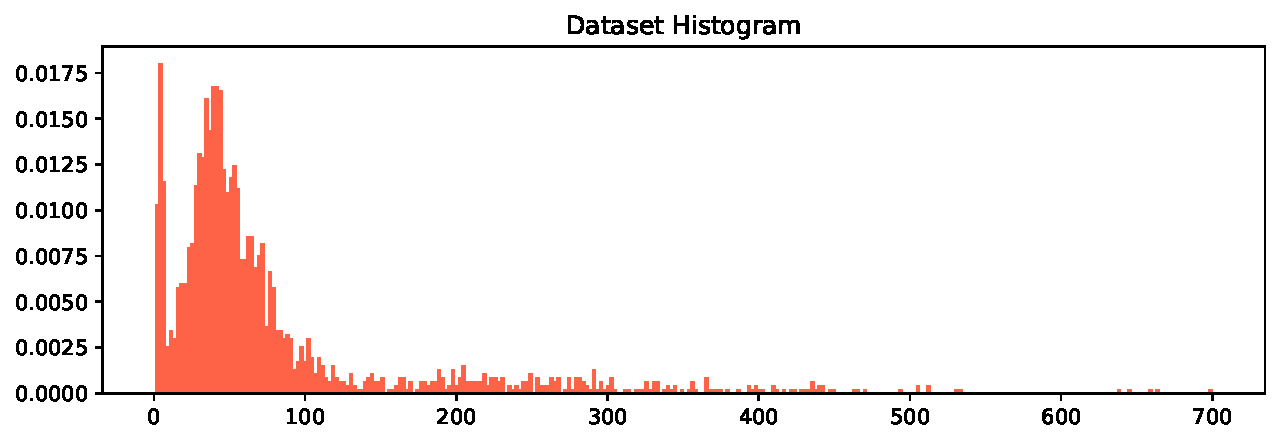
\includegraphics[scale=0.7]{figures/p2_1_dataset.pdf}
	\end{center}
	The distribution of the data appears to have 3 distinct peaks, a very sharp one centered at around $10$ hours, a high mass but slow falloff one at $50$ hours, and a very small flat peak at at 300 hours. A Gamma mixture model thus seems to be the perfect model for this distribution, since the distribution appears to be a mixture of several Gamma distribution with varying shape parameters.

	\begin{part}{2} Implement your solution from Problem 1 in \texttt{homework5.ipynb}.
	\end{part}

	% {\bfseries You will recieve no points for code not included below.}
	Using the formulas we derived in the previous problem, we get efficient functions using \texttt{scipy.stats} alongside \texttt{numpy} broadcasting features: (some code compressed for brevity)

	\begin{minted}{python}
  def e_step(theta, betas): # "q" estimation
    weighted_pdfs = theta * gamma.pdf(x, a=alpha, scale=1/betas)
    return weighted_pdfs / weighted_pdfs.sum(axis=1, keepdims=True)

  def m_step(q): # "theta", "betas" estimation
    return q.mean(axis=0), alpha * q.sum(axis=0) / (q * x).sum(axis=0)

  def log_likelihood(theta, betas):
      return np.log((theta * gamma.pdf(x, a=alpha, scale=1/betas)).sum(axis=1)).sum()

  def run_em(theta, betas, iterations=1000):
      for _ in range(iterations):
          q = e_step(theta, betas)
          theta, betas = m_step(q)

      return theta, betas
	\end{minted}

	\begin{part}{3} Run your code for 1, 2, 3, and 4 mixture components.  Plot the
		mixture models you find on top of the data distribution as well as
		the associated log likelihoods.  How many mixtures does it seem that
		there are?  How would you decide?
	\end{part}

	Using the code from the previous section, we get the following plots:
	\begin{center}
		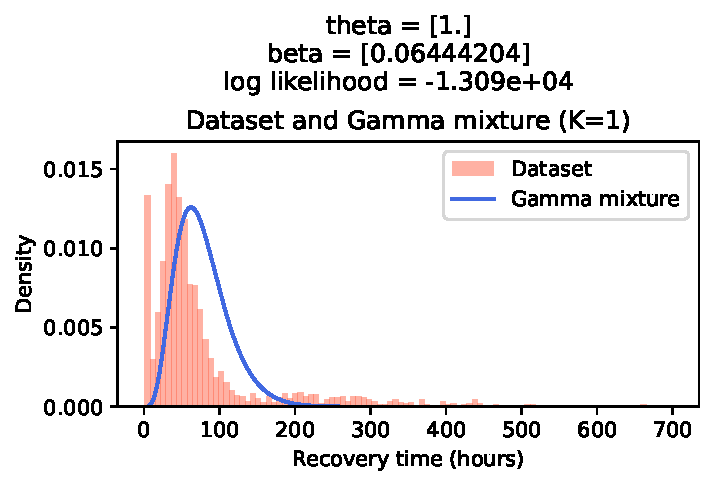
\includegraphics[scale=0.7]{figures/p2_3_1mixtures.pdf}
		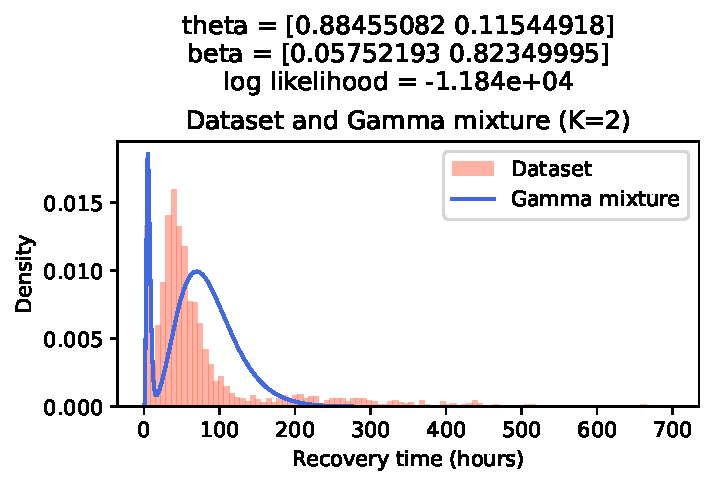
\includegraphics[scale=0.7]{figures/p2_3_2mixtures.pdf}

		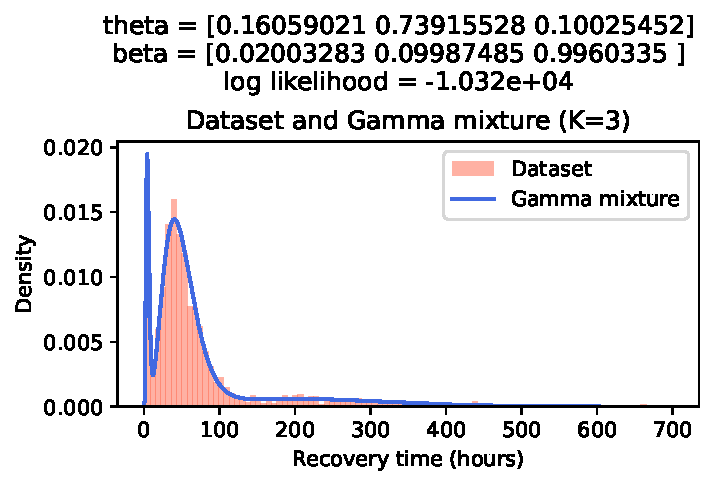
\includegraphics[scale=0.7]{figures/p2_3_3mixtures.pdf}
		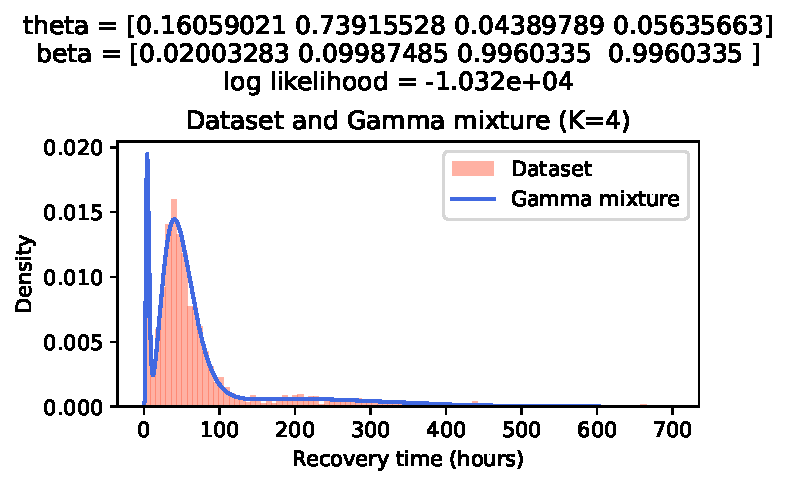
\includegraphics[scale=0.7]{figures/p2_3_4mixtures.pdf}
	\end{center}
	Graphing the log-likelihoods with respect to $K$, we get:
	\begin{center}
		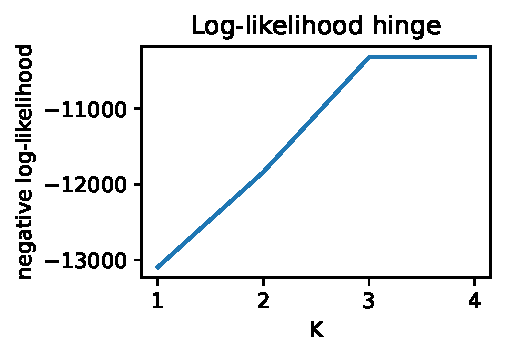
\includegraphics[scale=0.7]{figures/p2_3_hinge.pdf}
	\end{center}
	This readily-apparent hinge in the graph tells us that there are three mixtures, as we predicted. Put more simply, since the model completely stops improving after this point, there must be three mixtures.

	We can also see what happens when we add in a fourth model to the mixture to further understand why there are only 3 mixtures in the original data set. Here, we see by looking at the $\theta$ and $\beta$ parameters that the smallest Gamma distribution split into two smaller Gamma distributions when jumping from $K=3$ to $K=4$. Since this has no effect of the log-likelihood, such a splitting most likely does not represent the distribution of the underlying data.

	\begin{part}{4} The doctors tell you that a normal recovery from the procedure
		is about 2-3 days, though sometimes patients recover a little
		faster. Does this match what you see in the data?  Provide some
		hypotheses about what might be going on.
	\end{part}

	Yes, based on the three Gamma distributions in the mixture model, it seems that there are three different scenarios for recovery:
	\begin{enumerate}
		\item \textbf{Fast recovery:} A small number of patients recover within a half-day.
		\item \textbf{Medium recovery:} Most patients recover somewhere in the 1-3 day range.
		\item \textbf{Slow recovery:} A small number of patients take 1-3 weeks to recover.
	\end{enumerate}
	The doctors assessment is thus fairly accurate to what's reflected by the data.

	\begin{part}{5} It's clear from the data that some patients take significantly
		longer than 2-3 days.  Do you observe that there is evidence that
		these represent a different cluster, vs. a long tail from a single
		cluster?  Why or why not?
	\end{part}

	Yes. This longer tail does in fact come from a different distribution entirely to the main cluster. This can be seen since the log-likehood increased significantly when we add in the third distribution to the mixture model. Additionally, there is a notable, however slight, increase in the data past the decreasing tail of the main cluster.

	\begin{part}{6} The physician-scientists want to use this model to understand
		the characteristics of patients who have very long recoveries
		vs. those who do not.  Is this mixture modeling approach appropriate
		for this task?  Why or why not?
	\end{part}

	Yes, using a mixture model would be a great choice for this analysis, for a few reasons. First of all, we have no prior labels or understanding of the types of recovery mode, and the mixture model has successfully identified that there are in fact three different recovery distributions, and can separate these different recovery modes. This clear demarcation is especially useful for an unlabelled dataset such as the one we are given.

	\begin{part}{7} The physician-scientists develop a way of identifying someone's
		cluster based on a blood test -- it seems that some patients in the
		longer group are ones that are at risk for clotting-related
		complications.  The hospital operations staff want to use this model
		to help streamline operations.  They plan to use the cluster of the
		patient to predict which patients will have a long length of stay.
		Is this plan sound?  May there be some issues?
	\end{part}

	Using any learned model to allocate resources has understandable ethical concerns due to the severity of miscalculation, however with research and testing this might work. This blood test might be used in conjunction in the model to first of all verify its accuracy against the mixture model, and figure out the tolerances for error. Then the hospital could allocate beds more liberally than needed to avoid overcrowding. Overall, if its accuracy were demonstrated, the blood test might be a better indicator of recovery time than the mixture model, since the blood test might uncover the actual latent variables driving recovery time.
\end{parts}

\begin{problem}{3}[PCA]
For this problem you will implement PCA from scratch on the first 6000 images of the MNIST dataset. Your job is to apply PCA on MNIST and discuss what kind of structure is found.
\end{problem}

\begin{parts}
	\begin{part}{}
		Implement your solution in \texttt{homework5.ipynb} and attach the final plots below.
	\end{part}

	\begin{minted}{python}
  def pca(x, n_comps=500):
      _, S, U = np.linalg.svd(x - x.mean(axis=0), full_matrices=False)

      top_eigenvectors = Vt[:n_comps]
      top_eigenvalues = S[:n_comps] ** 2 / (x_centered.shape[0] - 1)
      
      return top_eigenvectors, top_eigenvalues 
  \end{minted}

	\begin{part}{1} Compute the PCA. Plot the eigenvalues corresponding to the most
		significant 500 components in order from most significant to
		least. Make another plot that describes the cumulative proportion of
		variance explained by the first $k$ most significant components for
		values of $k$ from 1 through 500.  How much variance is explained by
		the first 500 components?  Describe how the cumulative proportion of
		variance explained changes with $k$.  Include this plot below.
	\end{part}

	We use the following function to calculate the cumulative variance proportion:
	\begin{minted}{python}
  def calc_cfvs(eigvals):
      return np.cumsum(eigvals / np.sum(eigvals))
  \end{minted}

	Plotting the biggest $500$ eigenvalues alongside a graph of the cumulative variance proportion, we get:
	\begin{center}
		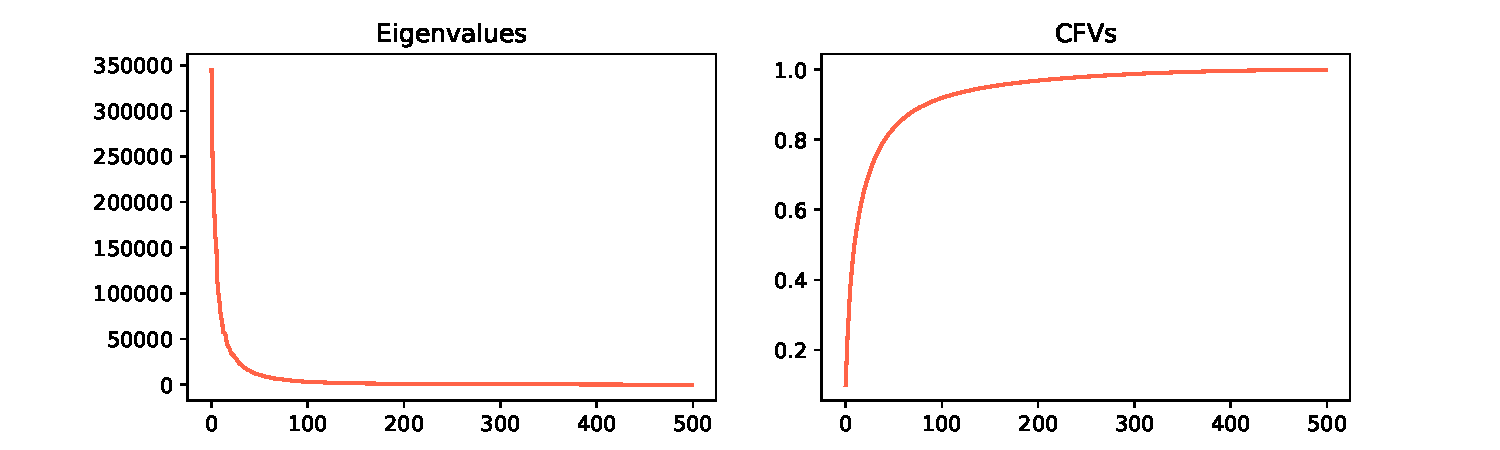
\includegraphics[scale=0.7]{figures/p3_cfvs.pdf}
	\end{center}
	The variance proportion explained by the first 500 components is $1.00$, meaning that the first 500 components are able to explain practically all of the variance. In actuality the variance proportion is $1 - \epsilon$ for some very small $\epsilon$, however due to numerical precision limits inherent in floating points, we are unable to measure this $\epsilon$ when $k=500$.

	It also seems that the eigenvalues roughly follow a Zipfian distribution. This means that the size of the eigenvalue is inversely proportional to it's index in the sorted array of eigenvalues. Correspondingly the cumulative variance proportion follows the Zipfian cumulative density function, which rapidly approaches $1$. Put into even simpler terms, it seems that the majority of variance is explained by a minority of the eigenvalues, and the shape/distribution of the cumulative variance proportion graph reflects this.

	\begin{part}{2} Plot the mean image of the dataset and plot an image
		corresponding to each of the first 10 principle components.  How do
		the principle component images compare to the cluster centers from
		K-means? Discuss any similarities and differences.  Include these
		two plots below.
	\end{part}

	Plotting the mean image, we get
	\begin{center}
		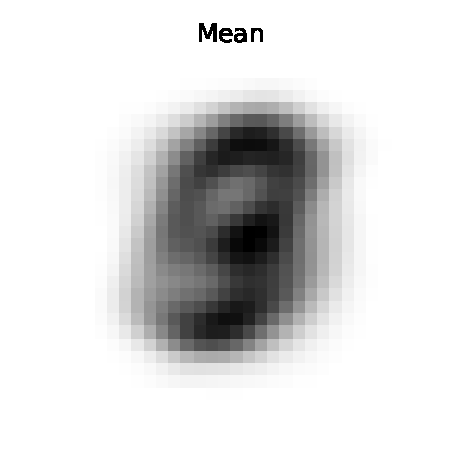
\includegraphics[scale=0.7]{figures/p3_mean.pdf}
	\end{center}
	This lines up with intuition -- most digits fit into an oval, are more concentrated towards the right, and have have a top, middle and bottom component.

	Plotting eigenvectors representing the first 10 principle components as images, we get:
	\begin{center}
		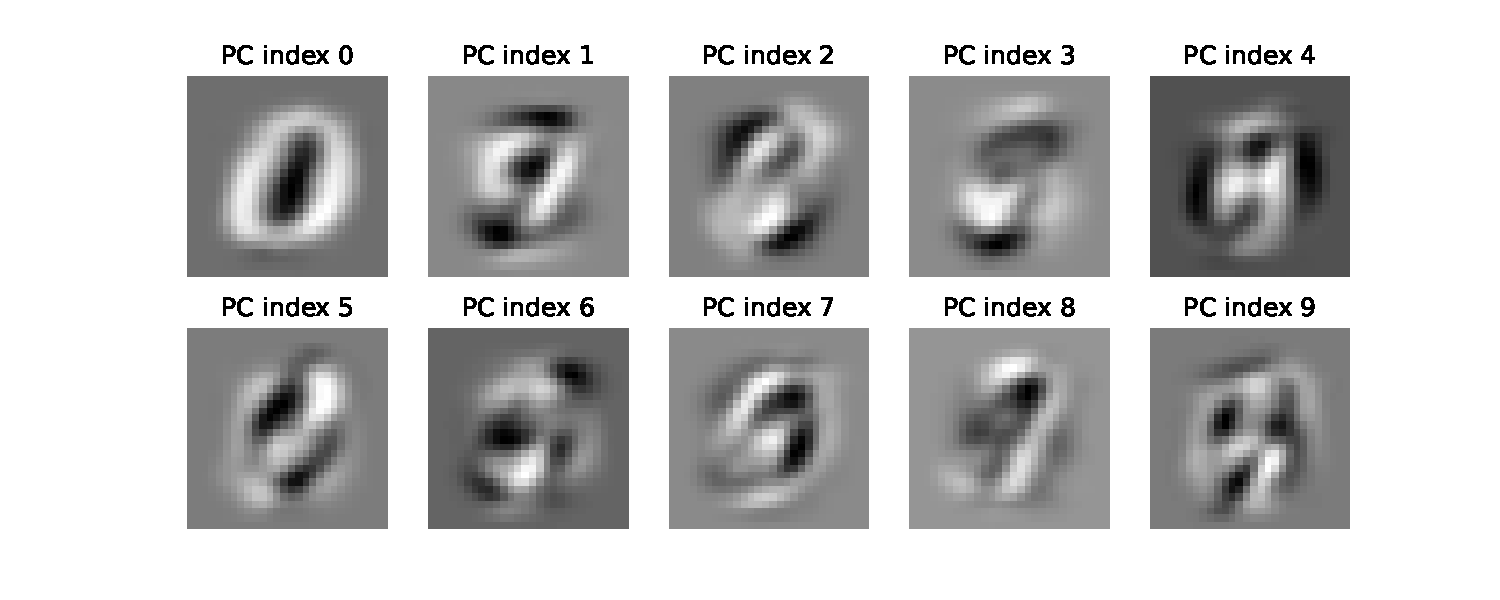
\includegraphics[scale=0.7]{figures/p3_pcomps.pdf}
	\end{center}
	Compared to the (standardized) K-means cluster centers from the previous problem set, these mean class images aren't as clearly associated to the ``true'' human classes. When looking at the (standardized) K-means clusters, it's fairly easy to identify most K-means cluster with a digit, or at least a visually distinct means of writing a digit. (For example, a looped 2 and an unlooped 2 were classified separately, but 3 and 8 were grouped together.) In the PCA components however, the only identifiable digits are 0 and maybe 9.

	A key similarity between PCA and K-means is how easily they are both able to detect the 0 digit, and perhaps this is due to it's visual distinction from the other digits. It also seems that PCA has a harder time understanding sharp edges -- all of the eigenvector images depict smoothly varying, blurred digits while K-means is able to pick representatives which have sharp edges, for instance in the 7-digit.

	\begin{part}{3} Compute the reconstruction error on the data set using the mean
		image of the dataset.  Then compute the reconstruction error using
		the first 10 principal components.  How do these errors compare to
		the final objective loss achieved by using K-means on the dataset?
		Discuss any similarities and differences. For consistency in grading, define the reconstruction error as the squared L2
		norm averaged over all data points.
	\end{part}

	We use the following code to calculate the reconstruction error:
	\begin{minted}{python}
  def calc_errs(x, pcomps):
      err_mean = ((x - x.mean(axis=0)) ** 2).sum(axis=1).mean()
      err_pcomp = ((x - np.dot(x, pcomps.T) @ pcomps) ** 2).sum(axis=1).mean()
      
      return err_mean, err_pcomp
	\end{minted}
	To compare this to K-means, we implement a similar method for our K-means clustering code from last problem set:
	\begin{minted}{python}
    def calc_errs_kmean(self, x):
        cluster_errors = [
            np.sum((x[self.cluster_assignments == k] - self.centroids[k])**2)
            for k in range(self.K)
        ]

        return np.array(cluster_errors).mean()
	\end{minted}
	As a sanity check, we note that a K-means reconstruction error for $K=1$ is the same as the mean error calculated in our PCA error method. Comparing the results of the PCA reconstruction error and K-means reconstruction error, we get

	\texttt{ Reconstruction error (mean): 3.436024e+06  }

	\texttt{ Reconstruction error (top 10 pcomps): 2.077421e+03  }

	\texttt{ Reconstruction error (K-means for K=10): 3.513074e+04 }

	Interestingly, PCA performs better at reconstruction than K-means on the MNIST dataset -- but only by an order of magnitude.

	\begin{part}{4}
		Suppose you took the original matrix of principle components
		that you found $U$ and multiplied it by some rotation matrix $R$.
		Would that change the quality of the reconstruction error in the
		last problem?  The interpretation of the components?  Why or why
		not?
	\end{part}

	Recall that if $U$ is the matrix of principal components, the reconstruction of a matrix of vectors $X$ is
	\[
		X_{\textrm{reconstructed}} = XU^\intercal U.
	\]
	If $R$ is some rotation matrix, which by definition satisfies $R^\intercal R = I$, and we replace $U$ by $RU$, we get
	\[
		X_{\textrm{reconstructed}}' = X(RU)^\intercal RU = XU^\intercal R^{\intercal} RU = XU^\intercal U = X_{\textrm{reconstructed}}.
	\]
	This means that the reconstruction error would not be altered if use \emph{all} principal component vectors. That being said such a rotation in principal component space would change the interpretation of each principal component vector. If originally each principal component vector represented an attribute of the dataset, after rotation these attributes might blend together so that each vector now represents a combination of attributes that might not be as easily interpretable. In particular, these rotated vectors might no longer be eigenvectors of the covariance matrix, and so don't necessarily correspond to the most significantly variant features of the dataset like the original principal component vectors do.

	This means that if we use only the top 10 principal components after rotation, the reconstruction error can only decrease since the original configuration minimizes reconstruction error. There are some rare circumstances where the reconstruction error wouldn't change -- for example if the rotation rotates one of the top eigenvectors 180 degrees around another, thus fixing the eigenspaces -- but generally any rotation would decrease the reconstruction error.

	\begin{part}{5}
		Let's recall the zipcode application in Homework 3.  A common
		application of PCA is to dimensionality reduction before running a
		classifier: You first project the data onto the first few PCA bases,
		and then you train a classifier from the projection to the output.
		How might this be better than associating digits to clusters, as you
		did in Homework 4?  Would this approach help with any of the attacks
		in Homework 3?
	\end{part}

	There are two main advantages that performing dimensionality reduction prior to running a classifier has over just running a classifier on the raw data. The first is noise reduction. Selecting just the top components of PCA significantly reduces the noise of the dataset since we remove many ``noisy features'' which usually have low variance. Reduced noise will naturally improve the performance of the classifier.

	The second advantage is reduced dimensionality. Many classifiers struggle with high-dimensional data -- this is known as the ``curse of dimensionality''. If the feature space is vast, the classifier might not be able to effectively learn discriminative patters. It also is more prone to overfitting in high dimensions -- especially when a high parameter model is trained on high-dimensional data. Reducing the dimensionality first mitigates both of these issues.

	In terms of mitigating against attacks, there are several advantages dimensionality reduction has in preventing certain attacks. A main useful feature is that dimensionality reduction reduces sensitivity to tiny perturbations which might be used in adversarial attacks. For other attacks such as changing hardware, model type, social engineering, etc, it's harder to see how reduced dimensionality could prevent such attacks.

	Finally, not only would dimensionality reduction improve classifier performance, but it would also improve runtime and memory usage due to the reduced amount of data which the classifier has to deal with. This would be crucial for high latency applications such as a fast zipcode reader.

	\begin{part}{6} You are collaborating with a penmanship analysis expert.  They
		are able to identify the kind of pen used to make a mark by various
		characteristics such as the width of the line, its crispness, and
		the type (if any) of ink splatter.  They have heard that your
		machine learning helped automate reading zip codes for the post
		office; they are wondering if you can help automate the manual
		process of classifying pen types.
	\end{part}
	\begin{parts}
		\begin{part}{} Does what the expert is describing correspond to some kind
			of hidden representation or latent variable?  Describe why or
			why not.
		\end{part}

		Yes, it seems based on the expert's description that the type of pen used when writing is a latent variable, since it generated many characteristics in the final data set such as line width, crispness, and type of ink splatter.

		\begin{part}{} Do you think PCA will help the expert?  Why or why not?
		\end{part}

		PCA might help as a tool, however due to the fine-grained nature of some of the data characteristics, it might make more sense to use PCA alongside other models such as convolutional neural networks. PCA, for example, might get rid of ink splatters and line crispness and instead focus more on the shape of the pen curves or percentage of the paper filled with ink. These are significant features, just not the ones we are looking for.

		A good alternative might be to pass the data through several learned filters (e.g. edge detection, convolving with some learned ink splatter kernel) and then performing PCA on the filtered data before passing through a classifier. This would give us the best of both worlds.
	\end{parts}
\end{parts}

\begin{problem}{4}[Bayesian Networks]
In this problem we explore the conditional independence
properties of a Bayesian Network.
Consider the following Bayesian
network representing a fictitious person's activities. Each random
variable is binary (true/false).

\medskip
% \begin{center}
% 	\begin{tikzpicture}[
% 			node distance=1cm and .5cm,
% 			bn/.style={draw,ellipse,text width=2cm,align=center}
% 		]
% 		\node[bn] (w) {\attr{Weekend}};
% 		\node[bn,below right=of w] (t) {\attr{Traveling}};
% 		\node[bn,right=of t] (s) {\attr{Sick}};
% 		\node[bn,below left=of w] (f) {\attr{Friends over}};
% 		\node[bn,below right=of f] (eef) {\attr{Eat exotic foods}};
% 		\node[bn,right=of eef] (gs) {\attr{Get sleep}};
% 		\path (w) edge[-latex] (t)
% 		(w) edge[-latex] (f)
% 		(f) edge[-latex] (eef)
% 		(t) edge[-latex] (eef)
% 		(t) edge[-latex] (gs)
% 		(s) edge[-latex] (gs)
% 		(s) edge[-latex] (eef);
% 	\end{tikzpicture}
% \end{center}

\begin{center}
	\begin{tikzpicture}[
		>={Latex[width=2mm,length=2mm]},
		state/.style={ellipse, draw, minimum width=2.5cm}
		]

		% Nodes
		\node[state] (weekend) {\attr{Weekend}};
		\node[state, below left=of weekend] (friends) {\attr{Friends over}};
		\node[state, below right=of weekend] (traveling) {\attr{Traveling}};
		\node[state, right=of traveling] (sick) {\attr{Sick}};
		\node[state, below=of friends] (food) {\attr{Eat exotic foods}};
		\node[state, below=of traveling] (sleep) {\attr{Get sleep}};

		% Paths
		\draw[->] (weekend) -- (friends);
		\draw[->] (weekend) -- (traveling);
		\draw[->] (sick) -- (food);
		\draw[->] (sick) -- (sleep);
		\draw[->] (traveling) -- (food);
		\draw[->] (traveling) -- (sleep);
		\draw[->] (friends) -- (food);

	\end{tikzpicture}
\end{center}

The random variables are:

\begin{itemize}
	\item \attr{Weekend}: Is it the weekend?
	\item \attr{Friends over}: Does the person have friends over?
	\item \attr{Traveling}: Is the person traveling?
	\item \attr{Sick}: Is the person sick?
	\item \attr{Eat exotic foods}: Is the person eating exotic foods?
	\item \attr{Get Sleep}: Is the person getting sleep?
\end{itemize}
\end{problem}

\begin{solution}
	For the following questions, $A \perp B$ means that events A and B are
	independent and $A \perp B \,|\, C$ means that events A and B are independent
	conditioned on C.

	\begin{part}{1}Is $\attr{Weekend} \perp \attr{Get Sleep}$?
		If NO, give intuition for why.
	\end{part}

	NO. The path $\attr{Weekend} \to \attr{Traveling} \to \attr{Get sleep}$ is not blocked, since we did not observe $\attr{Traveling}$.

	\begin{part}{2}Is $\attr{Sick} \perp \attr{Weekend}$?
		If NO, give intuition for why.
	\end{part}

	YES. Each path from $\attr{Sick}$ to $\attr{Weekend}$ is blocked by not observing $\attr{Eat exotic foods}$ and $\attr{Get sleep}$ respectively.

	\begin{part}{3}Is $\attr{Sick} \perp \attr{Friends over}\,\given\, \attr{Eat exotic
				foods}$? If NO, give intuition for why.
	\end{part}

	NO. The path $\attr{Sick} \to \attr{Eat exotic foods} \to \attr{Friends over}$ is not blocked since $\attr{Eat exotic foods}$ has been observed.

	\begin{part}{4}Is $\attr{Friends over} \perp \attr{Get Sleep}$? If NO, give
		intuition for why.
	\end{part}

	NO. The path $\attr{Friends over} \to \attr{Weekend} \to \attr{Traveling} \to \attr{Get Sleep}$ is not blocked since we observe neither $\attr{Weekend}$ nor $\attr{Traveling}$.

	\begin{part}{5} Is $\attr{Friends over} \perp \attr{Get Sleep} \given
			\attr{Traveling}$? If NO, give intuition for why.
	\end{part}

	YES. The path $\attr{Friends over} \to \attr{Weekend} \to \attr{Traveling} \to \attr{Get Sleep}$ is blocked by observing the event $\attr{Traveling}$, and the path $\attr{Friends over} \to \attr{Eat exotic foods} \to \attr{Sick} \to \attr{Get sleep}$ is blocked by not observing the event $\attr{Eat exotic foods}$.

	\begin{part}{6} Suppose the person stops traveling in ways that affect their
		sleep patterns.  Travel still
		affects whether they eat exotic foods.  Draw the modified network.
	\end{part}

	\begin{center}
		\begin{tikzpicture}[
			>={Latex[width=2mm,length=2mm]},
			state/.style={ellipse, draw, minimum width=2.5cm}
			]

			% Nodes
			\node[state] (weekend) {\attr{Weekend}};
			\node[state, below left=of weekend] (friends) {\attr{Friends over}};
			\node[state, below right=of weekend] (traveling) {\attr{Traveling}};
			\node[state, right=of traveling] (sick) {\attr{Sick}};
			\node[state, below=of friends] (food) {\attr{Eat exotic foods}};
			\node[state, below=of traveling] (sleep) {\attr{Get sleep}};

			% Paths
			\draw[->] (weekend) -- (friends);
			\draw[->] (weekend) -- (traveling);
			\draw[->] (sick) -- (food);
			\draw[->] (sick) -- (sleep);
			\draw[->] (traveling) -- (food);
			\draw[->] (friends) -- (food);
		\end{tikzpicture}
	\end{center}

	\begin{part}{7} For this modified network, is $\attr{Friends over} \perp
			\attr{Get sleep}$? If NO, give an intuition why.  If YES,
		describe what observations (if any) would cause them to no longer be
		independent.
	\end{part}

	YES. The path $\attr{Friends over} \to \attr{Eat exotic foods} \to \attr{Sick} \to \attr{Get sleep}$ is blocked by the event $\attr{Eat exotic foods}$ is not observed. If we observed the event $\attr{Eat exotic food}$, then $\attr{Friends over}$ would no longer be independent from $\attr{Get sleep}$.
\end{solution}
\end{document}
